\section{Introduction}
Social media has become a major source of information for analyzing
all aspects of daily life. In particular, public health monitoring can
now be conducted on Twitter in order to measure the wellbeing of
populations in different geographic regions. The ability to model
transitions for ailments and detect statements such as ``people talk
about smoking and cigarettes before talking about respiratory
problems'', or ``people talk about headaches and stomach ache in any
order'', has a range of applications in syndromic surveillance such as
measuring behavioral risk factors and triggering public health
campaigns. In this paper, we propose \tmatam, a method that models
temporal transitions that involve health-related topics. \tmatam
combines \atam, a latent health-related topic analysis method proposed
in~\cite{atam2}, with \tmlda, that models general-purpose topic
transitions~\cite{DBLP:conf/kdd/WangAB12}. We then propose \tatam,
a method which uncovers latent ailment inside tweets by treating
\texttt{\emph{time}} as a random variable inside
atam~\cite{atam2}.

Common ailments are continuously monitored by collecting data from
health care facilities, a process known as sentinel surveillance. Such
resources limit surveillance, most especially for real-time
feedback. For this reason, the Web has become a source of syndromic
surveillance, operating on a wider scale for a fraction of the
cost. While several latent topic modeling methods such as
Probabilistic Latent Semantic Indexing (pLSI)~\cite{plsi} and Latent
Dirichlet Allocation (LDA)~\cite{lda}, are used to effectively cluster
and classify general-purpose text, it has been shown that dedicated
methods such as the Ailment Topic Aspect Model (ATAM) are better
suited for capturing ailments in
Twitter~\cite{atam2}. ATAM extends LDA to model how users
express ailments in tweets. It assumes that each health-related tweet
reflects a latent ailment such as flu and allergies.  Similar to a
topic, an ailment indexes a word distribution. It also maintains a
distribution over symptoms and treatments. This level of detail
provides a more accurate model for latent ailments.

\begin{figure*}[t!]
\centering
\frame{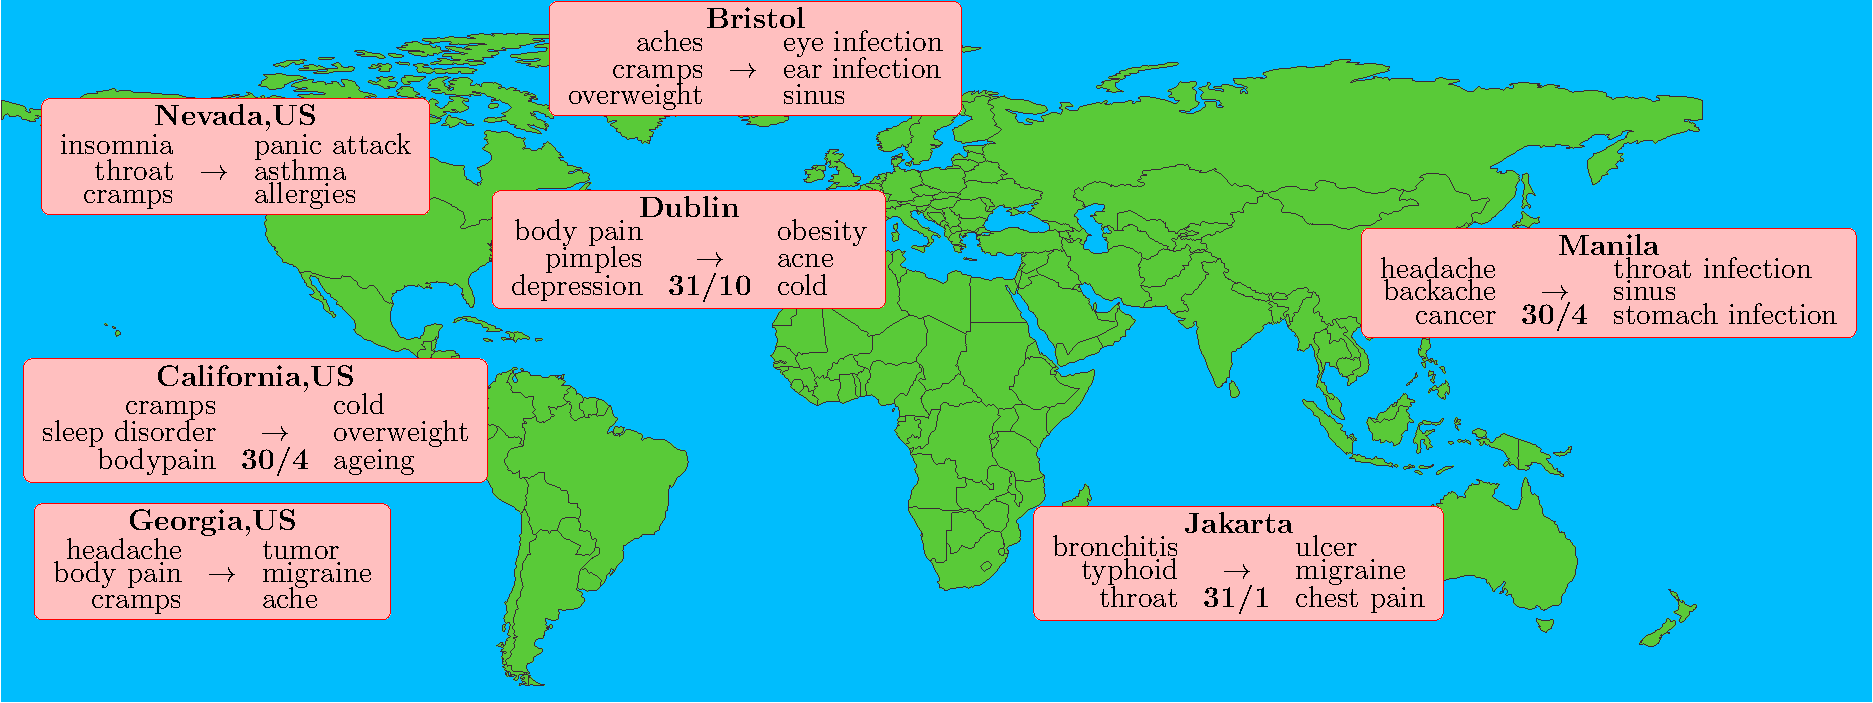
\includegraphics[width=0.80\textwidth]{tikz/eyecatcher.pdf}}
\caption{One-Way ailment transitions obtained by \tmatam for various 
regions. For each location the time period is divided into two parts, 
preceding and following the most significant change-point discovered
for that location. We show the most popular ailments on either 
side of this boundary.}
\label{fig:eyecatcher}
\end{figure*}

On the other hand, while pLSI and LDA have been shown to perform well
on static documents, they are not able to intrinsically capture topic
evolution over time.  Temporal-LDA (\tmlda) was hence proposed as an
extension to LDA for mining Twitter streams and providing effective
topic prediction over time~\cite{DBLP:conf/kdd/WangAB12}. In this
paper, we examine how well we can measure and predict ailment
transitions in Twitter by combining ATAM and TM-LDA into a new model,
coined \tmatam.  Just like \tmlda, \tmatam and \tatam are different from dynamic
topic models such as~\cite{DBLP:conf/icml/BleiL06}
and~\cite{DBLP:conf/icdm/LinMHJD11}, and from the work of Wang et
al.~\cite{DBLP:conf/kdd/WangM06}, as they are designed to learn topic
transition patterns from temporally-ordered posts, while dynamic topic
models focus on changing word distributions of topics over
time. \tmatam learns transition parameters that dictate the evolution
of health-related topics by minimizing the prediction error on ailment 
distributions of consecutive periods at different temporal and geographic 
granularities. \tatam on the other hand discovers latent ailments
in health tweets by treating time as a corpus-specific multinomial distribution.

Ailment distributions evolve over time. Further the evolution is
region-specific. While \tmatam and \tatam heavily borrow from ATAM and \tmlda,
their effectiveness require to carefully model two key granularities,
temporal and geographic. A temporal granularity that is too-fine may result in
sparse and spurious transitions whereas a too-coarse one could miss
valuable ailment transitions. Similarly, a too-fine geographic
granularity may produce false positives and a too coarse one may cover
a user population that is exposed to different weather conditions and
miss meaningful transitions. For example, it has been shown that discussions on
allergies break at different periods in different states in the
USA~\cite{atam2}. Therefore, processing all tweets originating from the USA together
will miss climate variations that affect people's health. We argue
for the need to consider different time granularities for different
regions and we wish to identify and model the evolution of ailment
distributions between different temporal granularities.

Our experiments on a corpus of more than $500K$ health-related tweets
collected over a period of 8 months show that \tmatam outperforms
\tmlda in estimating temporal topic transitions of different
geographic populations. Our results can be classified in 2 kinds of
transitions. {\selftransitions} are those where a health-related topic
is mentioned continuously. {\em One-Way transitions} cover the case where
some topics are discussed after others. For example, our
study of tweets from California revealed many self transitions such as
headaches and migraines. On the other hand, tweeting about smoking,
drugs and cigarettes is followed by tweeting about respiratory
ailments. Figure~\ref{fig:eyecatcher} shows example one-way transitions we extracted for different states and cities in the
world. Such transitions are often due to external factors such as climate, health campaigns, nutrition and lifestyle of different world populations.

The outline of the paper is as follows: in
Section~\ref{sec:background} we first introduce the key ingredients of 
our data model, and then present the necessary background on
topic modeling (\lda, \atam). Finally we formalize the ailment prediction
problem. In Section~\ref{sec:approach}, we describe the construction of \tmatam and \tatam.
In Section~\ref{sec:results} we present the experiments designed to study
the behavior and performance of \tmatam and \tatam. Related work is overviewed in 
Section~\ref{sec:relwork}. We conclude and give some perspectives for 
future work in Section~\ref{sec:conclusion}.
